\documentclass[1p]{elsarticle_modified}
%\bibliographystyle{elsarticle-num}

%\usepackage[colorlinks]{hyperref}
%\usepackage{abbrmath_seonhwa} %\Abb, \Ascr, \Acal ,\Abf, \Afrak
\usepackage{amsfonts}
\usepackage{amssymb}
\usepackage{amsmath}
\usepackage{amsthm}
\usepackage{scalefnt}
\usepackage{amsbsy}
\usepackage{kotex}
\usepackage{caption}
\usepackage{subfig}
\usepackage{color}
\usepackage{graphicx}
\usepackage{xcolor} %% white, black, red, green, blue, cyan, magenta, yellow
\usepackage{float}
\usepackage{setspace}
\usepackage{hyperref}

\usepackage{tikz}
\usetikzlibrary{arrows}

\usepackage{multirow}
\usepackage{array} % fixed length table
\usepackage{hhline}

%%%%%%%%%%%%%%%%%%%%%
\makeatletter
\renewcommand*\env@matrix[1][\arraystretch]{%
	\edef\arraystretch{#1}%
	\hskip -\arraycolsep
	\let\@ifnextchar\new@ifnextchar
	\array{*\c@MaxMatrixCols c}}
\makeatother %https://tex.stackexchange.com/questions/14071/how-can-i-increase-the-line-spacing-in-a-matrix
%%%%%%%%%%%%%%%

\usepackage[normalem]{ulem}

\newcommand{\msout}[1]{\ifmmode\text{\sout{\ensuremath{#1}}}\else\sout{#1}\fi}
%SOURCE: \msout is \stkout macro in https://tex.stackexchange.com/questions/20609/strikeout-in-math-mode

\newcommand{\cancel}[1]{
	\ifmmode
	{\color{red}\msout{#1}}
	\else
	{\color{red}\sout{#1}}
	\fi
}

\newcommand{\add}[1]{
	{\color{blue}\uwave{#1}}
}

\newcommand{\replace}[2]{
	\ifmmode
	{\color{red}\msout{#1}}{\color{blue}\uwave{#2}}
	\else
	{\color{red}\sout{#1}}{\color{blue}\uwave{#2}}
	\fi
}

\newcommand{\Sol}{\mathcal{S}} %segment
\newcommand{\D}{D} %diagram
\newcommand{\A}{\mathcal{A}} %arc


%%%%%%%%%%%%%%%%%%%%%%%%%%%%%5 test

\def\sl{\operatorname{\textup{SL}}(2,\Cbb)}
\def\psl{\operatorname{\textup{PSL}}(2,\Cbb)}
\def\quan{\mkern 1mu \triangleright \mkern 1mu}

\theoremstyle{definition}
\newtheorem{thm}{Theorem}[section]
\newtheorem{prop}[thm]{Proposition}
\newtheorem{lem}[thm]{Lemma}
\newtheorem{ques}[thm]{Question}
\newtheorem{cor}[thm]{Corollary}
\newtheorem{defn}[thm]{Definition}
\newtheorem{exam}[thm]{Example}
\newtheorem{rmk}[thm]{Remark}
\newtheorem{alg}[thm]{Algorithm}

\newcommand{\I}{\sqrt{-1}}
\begin{document}

%\begin{frontmatter}
%
%\title{Boundary parabolic representations of knots up to 8 crossings}
%
%%% Group authors per affiliation:
%\author{Yunhi Cho} 
%\address{Department of Mathematics, University of Seoul, Seoul, Korea}
%\ead{yhcho@uos.ac.kr}
%
%
%\author{Seonhwa Kim} %\fnref{s_kim}}
%\address{Center for Geometry and Physics, Institute for Basic Science, Pohang, 37673, Korea}
%\ead{ryeona17@ibs.re.kr}
%
%\author{Hyuk Kim}
%\address{Department of Mathematical Sciences, Seoul National University, Seoul 08826, Korea}
%\ead{hyukkim@snu.ac.kr}
%
%\author{Seokbeom Yoon}
%\address{Department of Mathematical Sciences, Seoul National University, Seoul, 08826,  Korea}
%\ead{sbyoon15@snu.ac.kr}
%
%\begin{abstract}
%We find all boundary parabolic representation of knots up to 8 crossings.
%
%\end{abstract}
%\begin{keyword}
%    \MSC[2010] 57M25 
%\end{keyword}
%
%\end{frontmatter}

%\linenumbers
%\tableofcontents
%
\newcommand\colored[1]{\textcolor{white}{\rule[-0.35ex]{0.8em}{1.4ex}}\kern-0.8em\color{red} #1}%
%\newcommand\colored[1]{\textcolor{white}{ #1}\kern-2.17ex	\textcolor{white}{ #1}\kern-1.81ex	\textcolor{white}{ #1}\kern-2.15ex\color{red}#1	}

{\Large $\underline{12n_{0822}~(K12n_{0822})}$}

\setlength{\tabcolsep}{10pt}
\renewcommand{\arraystretch}{1.6}
\vspace{1cm}\begin{tabular}{m{100pt}>{\centering\arraybackslash}m{274pt}}
\multirow{5}{120pt}{
	\centering
	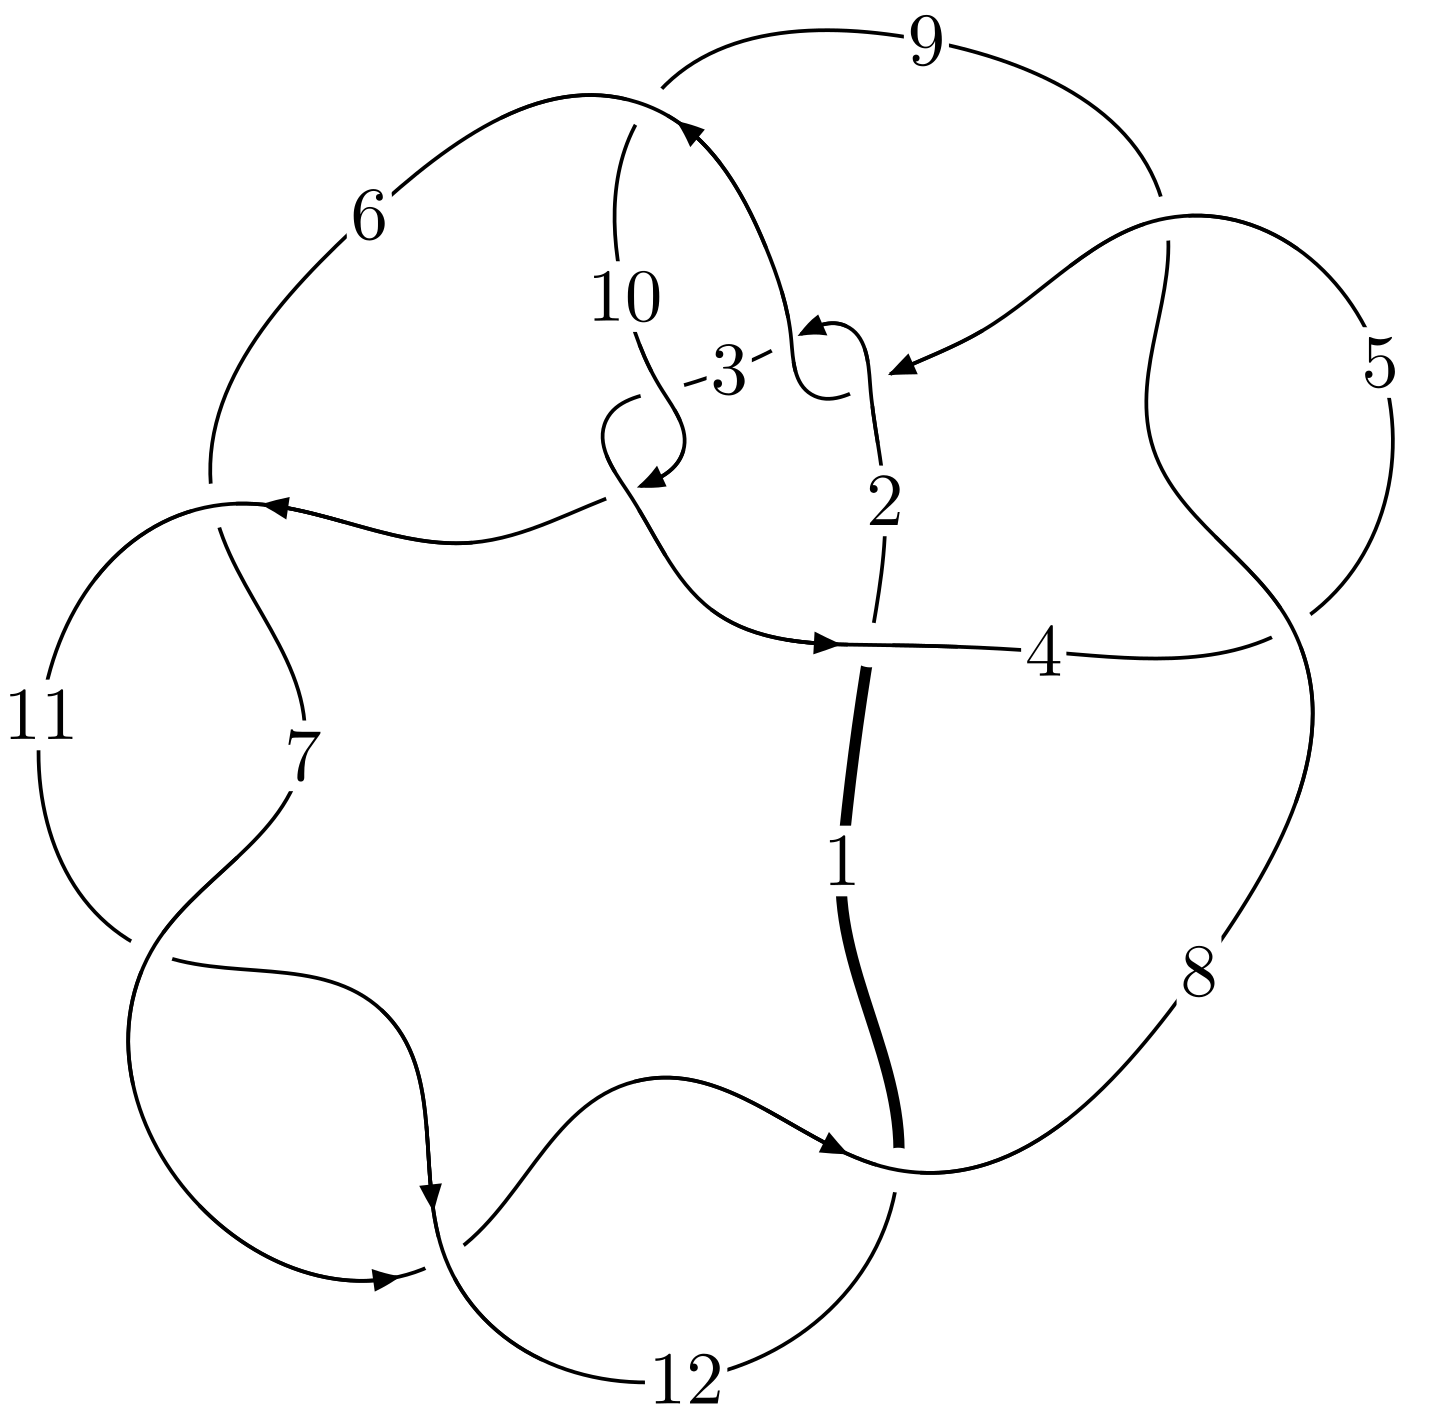
\includegraphics[width=112pt]{../../../GIT/diagram.site/Diagrams/png/2911_12n_0822.png}\\
\ \ \ A knot diagram\footnotemark}&
\allowdisplaybreaks
\textbf{Linearized knot diagam} \\
\cline{2-2}
 &
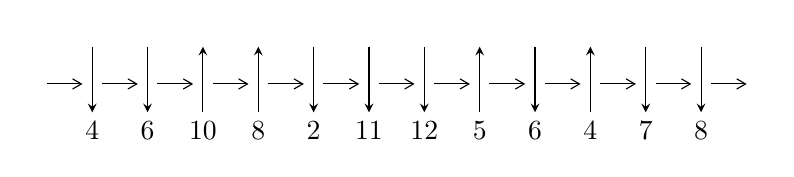
\begin{tikzpicture}[x=20pt, y=17pt]
	% nodes
	\node (C0) at (0, 0) {};
	\node (C1) at (1, 0) {};
	\node (C1U) at (1, +1) {};
	\node (C1D) at (1, -1) {4};

	\node (C2) at (2, 0) {};
	\node (C2U) at (2, +1) {};
	\node (C2D) at (2, -1) {6};

	\node (C3) at (3, 0) {};
	\node (C3U) at (3, +1) {};
	\node (C3D) at (3, -1) {10};

	\node (C4) at (4, 0) {};
	\node (C4U) at (4, +1) {};
	\node (C4D) at (4, -1) {8};

	\node (C5) at (5, 0) {};
	\node (C5U) at (5, +1) {};
	\node (C5D) at (5, -1) {2};

	\node (C6) at (6, 0) {};
	\node (C6U) at (6, +1) {};
	\node (C6D) at (6, -1) {11};

	\node (C7) at (7, 0) {};
	\node (C7U) at (7, +1) {};
	\node (C7D) at (7, -1) {12};

	\node (C8) at (8, 0) {};
	\node (C8U) at (8, +1) {};
	\node (C8D) at (8, -1) {5};

	\node (C9) at (9, 0) {};
	\node (C9U) at (9, +1) {};
	\node (C9D) at (9, -1) {6};

	\node (C10) at (10, 0) {};
	\node (C10U) at (10, +1) {};
	\node (C10D) at (10, -1) {4};

	\node (C11) at (11, 0) {};
	\node (C11U) at (11, +1) {};
	\node (C11D) at (11, -1) {7};

	\node (C12) at (12, 0) {};
	\node (C12U) at (12, +1) {};
	\node (C12D) at (12, -1) {8};
	\node (C13) at (13, 0) {};

	% arrows
	\draw[->,>={angle 60}]
	(C0) edge (C1) (C1) edge (C2) (C2) edge (C3) (C3) edge (C4) (C4) edge (C5) (C5) edge (C6) (C6) edge (C7) (C7) edge (C8) (C8) edge (C9) (C9) edge (C10) (C10) edge (C11) (C11) edge (C12) (C12) edge (C13) ;	\draw[->,>=stealth]
	(C1U) edge (C1D) (C2U) edge (C2D) (C3D) edge (C3U) (C4D) edge (C4U) (C5U) edge (C5D) (C6U) edge (C6D) (C7U) edge (C7D) (C8D) edge (C8U) (C9U) edge (C9D) (C10D) edge (C10U) (C11U) edge (C11D) (C12U) edge (C12D) ;
	\end{tikzpicture} \\
\hhline{~~} \\& 
\textbf{Solving Sequence} \\ \cline{2-2} 
 &
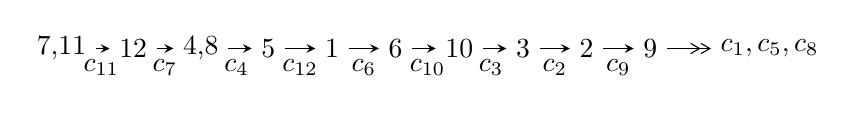
\begin{tikzpicture}[x=23pt, y=7pt]
	% node
	\node (A0) at (-1/8, 0) {7,11};
	\node (A1) at (1, 0) {12};
	\node (A2) at (33/16, 0) {4,8};
	\node (A3) at (25/8, 0) {5};
	\node (A4) at (33/8, 0) {1};
	\node (A5) at (41/8, 0) {6};
	\node (A6) at (49/8, 0) {10};
	\node (A7) at (57/8, 0) {3};
	\node (A8) at (65/8, 0) {2};
	\node (A9) at (73/8, 0) {9};
	\node (C1) at (1/2, -1) {$c_{11}$};
	\node (C2) at (3/2, -1) {$c_{7}$};
	\node (C3) at (21/8, -1) {$c_{4}$};
	\node (C4) at (29/8, -1) {$c_{12}$};
	\node (C5) at (37/8, -1) {$c_{6}$};
	\node (C6) at (45/8, -1) {$c_{10}$};
	\node (C7) at (53/8, -1) {$c_{3}$};
	\node (C8) at (61/8, -1) {$c_{2}$};
	\node (C9) at (69/8, -1) {$c_{9}$};
	\node (A10) at (11, 0) {$c_{1},c_{5},c_{8}$};

	% edge
	\draw[->,>=stealth]	
	(A0) edge (A1) (A1) edge (A2) (A2) edge (A3) (A3) edge (A4) (A4) edge (A5) (A5) edge (A6) (A6) edge (A7) (A7) edge (A8) (A8) edge (A9) ;
	\draw[->>,>={angle 60}]	
	(A9) edge (A10);
\end{tikzpicture} \\ 

\end{tabular} \\

\footnotetext{
The image of knot diagram is generated by the software ``\textbf{Draw programme}" developed by Andrew Bartholomew(\url{http://www.layer8.co.uk/maths/draw/index.htm\#Running-draw}), where we modified some parts for our purpose(\url{https://github.com/CATsTAILs/LinksPainter}).
}\phantom \\ \newline 
\centering \textbf{Ideals for irreducible components\footnotemark of $X_{\text{par}}$} 
 
\begin{align*}
I^u_{1}&=\langle 
-3 u^{15}+14 u^{14}+\cdots+2 b+10,\;-21 u^{15}+100 u^{14}+\cdots+4 a+68,\;u^{16}-6 u^{15}+\cdots+2 u+4\rangle \\
I^u_{2}&=\langle 
475 u^4 a^3-65 u^4 a^2+\cdots+311 a+1939,\;- u^4 a^3+2 u^4 a^2+\cdots-2 a+1,\;u^5+u^4-2 u^3- u^2+u-1\rangle \\
I^u_{3}&=\langle 
u^4-3 u^2+b+1,\;u^7-6 u^5+u^4+11 u^3-3 u^2+a-6 u+1,\\
\phantom{I^u_{3}}&\phantom{= \langle  }u^9+u^8-6 u^7-5 u^6+12 u^5+7 u^4-9 u^3-2 u^2+u-1\rangle \\
\\
\end{align*}
\raggedright * 3 irreducible components of $\dim_{\mathbb{C}}=0$, with total 45 representations.\\
\footnotetext{All coefficients of polynomials are rational numbers. But the coefficients are sometimes approximated in decimal forms when there is not enough margin.}
\newpage
\renewcommand{\arraystretch}{1}
\centering \section*{I. $I^u_{1}= \langle -3 u^{15}+14 u^{14}+\cdots+2 b+10,\;-21 u^{15}+100 u^{14}+\cdots+4 a+68,\;u^{16}-6 u^{15}+\cdots+2 u+4 \rangle$}
\flushleft \textbf{(i) Arc colorings}\\
\begin{tabular}{m{7pt} m{180pt} m{7pt} m{180pt} }
\flushright $a_{7}=$&$\begin{pmatrix}0\\u\end{pmatrix}$ \\
\flushright $a_{11}=$&$\begin{pmatrix}1\\0\end{pmatrix}$ \\
\flushright $a_{12}=$&$\begin{pmatrix}1\\u^2\end{pmatrix}$ \\
\flushright $a_{4}=$&$\begin{pmatrix}\frac{21}{4} u^{15}-25 u^{14}+\cdots-\frac{99}{4} u-17\\\frac{3}{2} u^{15}-7 u^{14}+\cdots-\frac{13}{2} u-5\end{pmatrix}$ \\
\flushright $a_{8}=$&$\begin{pmatrix}- u\\- u^3+u\end{pmatrix}$ \\
\flushright $a_{5}=$&$\begin{pmatrix}\frac{13}{4} u^{15}-16 u^{14}+\cdots-\frac{67}{4} u-11\\-\frac{3}{2} u^{15}+5 u^{14}+\cdots-\frac{1}{2} u+1\end{pmatrix}$ \\
\flushright $a_{1}=$&$\begin{pmatrix}- u^2+1\\- u^4+2 u^2\end{pmatrix}$ \\
\flushright $a_{6}=$&$\begin{pmatrix}u\\u\end{pmatrix}$ \\
\flushright $a_{10}=$&$\begin{pmatrix}\frac{3}{2} u^{15}-\frac{11}{2} u^{14}+\cdots-\frac{3}{2} u-\frac{3}{2}\\\frac{7}{2} u^{15}-15 u^{14}+\cdots-\frac{15}{2} u-8\end{pmatrix}$ \\
\flushright $a_{3}=$&$\begin{pmatrix}\frac{25}{2} u^{15}-\frac{113}{2} u^{14}+\cdots-\frac{85}{2} u-\frac{67}{2}\\\frac{19}{2} u^{15}-43 u^{14}+\cdots-\frac{61}{2} u-26\end{pmatrix}$ \\
\flushright $a_{2}=$&$\begin{pmatrix}\frac{11}{2} u^{15}-\frac{51}{2} u^{14}+\cdots-\frac{43}{2} u-\frac{31}{2}\\\frac{5}{2} u^{15}-12 u^{14}+\cdots-\frac{19}{2} u-8\end{pmatrix}$ \\
\flushright $a_{9}=$&$\begin{pmatrix}\frac{9}{2} u^{15}-\frac{41}{2} u^{14}+\cdots-\frac{29}{2} u-\frac{23}{2}\\\frac{13}{2} u^{15}-30 u^{14}+\cdots-\frac{41}{2} u-18\end{pmatrix}$\\&\end{tabular}
\flushleft \textbf{(ii) Obstruction class $= -1$}\\~\\
\flushleft \textbf{(iii) Cusp Shapes $= -11 u^{15}+53 u^{14}-38 u^{13}-147 u^{12}+140 u^{11}+198 u^{10}+121 u^9-664 u^8-111 u^7+438 u^6+477 u^5-133 u^4-460 u^3+26 u^2+46 u+30$}\\~\\
\newpage\renewcommand{\arraystretch}{1}
\flushleft \textbf{(iv) u-Polynomials at the component}\newline \\
\begin{tabular}{m{50pt}|m{274pt}}
Crossings & \hspace{64pt}u-Polynomials at each crossing \\
\hline $$\begin{aligned}c_{1}\end{aligned}$$&$\begin{aligned}
&u^{16}+2 u^{15}+\cdots-6 u+1
\end{aligned}$\\
\hline $$\begin{aligned}c_{2},c_{5}\end{aligned}$$&$\begin{aligned}
&u^{16}+13 u^{15}+\cdots+208 u+32
\end{aligned}$\\
\hline $$\begin{aligned}c_{3},c_{4},c_{8}\\c_{10}\end{aligned}$$&$\begin{aligned}
&u^{16}- u^{15}+\cdots+u+1
\end{aligned}$\\
\hline $$\begin{aligned}c_{6},c_{7},c_{11}\\c_{12}\end{aligned}$$&$\begin{aligned}
&u^{16}-6 u^{15}+\cdots+2 u+4
\end{aligned}$\\
\hline $$\begin{aligned}c_{9}\end{aligned}$$&$\begin{aligned}
&u^{16}- u^{15}+\cdots-15 u+1
\end{aligned}$\\
\hline
\end{tabular}\\~\\
\newpage\renewcommand{\arraystretch}{1}
\flushleft \textbf{(v) Riley Polynomials at the component}\newline \\
\begin{tabular}{m{50pt}|m{274pt}}
Crossings & \hspace{64pt}Riley Polynomials at each crossing \\
\hline $$\begin{aligned}c_{1}\end{aligned}$$&$\begin{aligned}
&y^{16}+22 y^{15}+\cdots-52 y+1
\end{aligned}$\\
\hline $$\begin{aligned}c_{2},c_{5}\end{aligned}$$&$\begin{aligned}
&y^{16}-5 y^{15}+\cdots-5888 y+1024
\end{aligned}$\\
\hline $$\begin{aligned}c_{3},c_{4},c_{8}\\c_{10}\end{aligned}$$&$\begin{aligned}
&y^{16}-19 y^{15}+\cdots-7 y+1
\end{aligned}$\\
\hline $$\begin{aligned}c_{6},c_{7},c_{11}\\c_{12}\end{aligned}$$&$\begin{aligned}
&y^{16}-18 y^{15}+\cdots-60 y+16
\end{aligned}$\\
\hline $$\begin{aligned}c_{9}\end{aligned}$$&$\begin{aligned}
&y^{16}+27 y^{15}+\cdots-229 y+1
\end{aligned}$\\
\hline
\end{tabular}\\~\\
\newpage\flushleft \textbf{(vi) Complex Volumes and Cusp Shapes}
$$\begin{array}{c|c|c}  
\text{Solutions to }I^u_{1}& \I (\text{vol} + \sqrt{-1}CS) & \text{Cusp shape}\\
 \hline 
\begin{aligned}
u &= -0.526647 + 0.921315 I \\
a &= -0.158275 + 0.852282 I \\
b &= \phantom{-}1.61938 + 0.26122 I\end{aligned}
 & \phantom{-}12.5756 + 7.7658 I & -0.37746 - 4.72182 I \\ \hline\begin{aligned}
u &= -0.526647 - 0.921315 I \\
a &= -0.158275 - 0.852282 I \\
b &= \phantom{-}1.61938 - 0.26122 I\end{aligned}
 & \phantom{-}12.5756 - 7.7658 I & -0.37746 + 4.72182 I \\ \hline\begin{aligned}
u &= -0.641134 + 0.907508 I \\
a &= -0.131631 - 0.748203 I \\
b &= -1.57975 + 0.10158 I\end{aligned}
 & \phantom{-}12.24930 - 1.78364 I & -0.280416 + 0.020773 I \\ \hline\begin{aligned}
u &= -0.641134 - 0.907508 I \\
a &= -0.131631 + 0.748203 I \\
b &= -1.57975 - 0.10158 I\end{aligned}
 & \phantom{-}12.24930 + 1.78364 I & -0.280416 - 0.020773 I \\ \hline\begin{aligned}
u &= -0.860541\phantom{ +0.000000I} \\
a &= \phantom{-}0.313373\phantom{ +0.000000I} \\
b &= \phantom{-}0.501732\phantom{ +0.000000I}\end{aligned}
 & -1.66742\phantom{ +0.000000I} & -3.52050\phantom{ +0.000000I} \\ \hline\begin{aligned}
u &= \phantom{-}1.384200 + 0.067843 I \\
a &= -0.23731 - 1.57085 I \\
b &= \phantom{-}0.063351 - 0.856630 I\end{aligned}
 & -5.42049 - 2.20486 I & -9.58545 + 3.34239 I \\ \hline\begin{aligned}
u &= \phantom{-}1.384200 - 0.067843 I \\
a &= -0.23731 + 1.57085 I \\
b &= \phantom{-}0.063351 + 0.856630 I\end{aligned}
 & -5.42049 + 2.20486 I & -9.58545 - 3.34239 I \\ \hline\begin{aligned}
u &= \phantom{-}0.536874\phantom{ +0.000000I} \\
a &= -1.68270\phantom{ +0.000000I} \\
b &= \phantom{-}0.418387\phantom{ +0.000000I}\end{aligned}
 & -2.43643\phantom{ +0.000000I} & \phantom{-}6.61560\phantom{ +0.000000I} \\ \hline\begin{aligned}
u &= \phantom{-}1.54541 + 0.35416 I \\
a &= -0.78815 + 1.39880 I \\
b &= -1.60127 + 0.41996 I\end{aligned}
 & \phantom{-}5.91450 - 12.45070 I & -3.55733 + 5.83875 I \\ \hline\begin{aligned}
u &= \phantom{-}1.54541 - 0.35416 I \\
a &= -0.78815 - 1.39880 I \\
b &= -1.60127 - 0.41996 I\end{aligned}
 & \phantom{-}5.91450 + 12.45070 I & -3.55733 - 5.83875 I\\
 \hline 
 \end{array}$$\newpage$$\begin{array}{c|c|c}  
\text{Solutions to }I^u_{1}& \I (\text{vol} + \sqrt{-1}CS) & \text{Cusp shape}\\
 \hline 
\begin{aligned}
u &= -0.252945 + 0.318927 I \\
a &= \phantom{-}0.736930 - 0.632401 I \\
b &= -0.145126 - 0.490024 I\end{aligned}
 & -0.252639 + 0.904244 I & -5.12440 - 7.64172 I \\ \hline\begin{aligned}
u &= -0.252945 - 0.318927 I \\
a &= \phantom{-}0.736930 + 0.632401 I \\
b &= -0.145126 + 0.490024 I\end{aligned}
 & -0.252639 - 0.904244 I & -5.12440 + 7.64172 I \\ \hline\begin{aligned}
u &= -1.65011\phantom{ +0.000000I} \\
a &= -0.204743\phantom{ +0.000000I} \\
b &= -0.895334\phantom{ +0.000000I}\end{aligned}
 & -10.2599\phantom{ +0.000000I} & -6.17920\phantom{ +0.000000I} \\ \hline\begin{aligned}
u &= \phantom{-}1.62313 + 0.35288 I \\
a &= \phantom{-}0.898424 - 0.854793 I \\
b &= \phantom{-}1.47438 - 0.04596 I\end{aligned}
 & \phantom{-}4.87833 - 2.98005 I & -2.44851 + 1.44008 I \\ \hline\begin{aligned}
u &= \phantom{-}1.62313 - 0.35288 I \\
a &= \phantom{-}0.898424 + 0.854793 I \\
b &= \phantom{-}1.47438 + 0.04596 I\end{aligned}
 & \phantom{-}4.87833 + 2.98005 I & -2.44851 - 1.44008 I \\ \hline\begin{aligned}
u &= \phantom{-}1.70974\phantom{ +0.000000I} \\
a &= -0.565907\phantom{ +0.000000I} \\
b &= -0.686707\phantom{ +0.000000I}\end{aligned}
 & -10.9818\phantom{ +0.000000I} & \phantom{-}0.831250\phantom{ +0.000000I}\\
 \hline 
 \end{array}$$\newpage\newpage\renewcommand{\arraystretch}{1}
\centering \section*{II. $I^u_{2}= \langle 475 u^4 a^3-65 u^4 a^2+\cdots+311 a+1939,\;- u^4 a^3+2 u^4 a^2+\cdots-2 a+1,\;u^5+u^4-2 u^3- u^2+u-1 \rangle$}
\flushleft \textbf{(i) Arc colorings}\\
\begin{tabular}{m{7pt} m{180pt} m{7pt} m{180pt} }
\flushright $a_{7}=$&$\begin{pmatrix}0\\u\end{pmatrix}$ \\
\flushright $a_{11}=$&$\begin{pmatrix}1\\0\end{pmatrix}$ \\
\flushright $a_{12}=$&$\begin{pmatrix}1\\u^2\end{pmatrix}$ \\
\flushright $a_{4}=$&$\begin{pmatrix}a\\-0.304292 a^{3} u^{4}+0.0416400 a^{2} u^{4}+\cdots-0.199231 a-1.24215\end{pmatrix}$ \\
\flushright $a_{8}=$&$\begin{pmatrix}- u\\- u^3+u\end{pmatrix}$ \\
\flushright $a_{5}=$&$\begin{pmatrix}-0.136451 a^{3} u^{4}+0.502883 a^{2} u^{4}+\cdots+0.516976 a+0.152466\\-0.431134 a^{3} u^{4}+0.227418 a^{2} u^{4}+\cdots+0.450352 a-1.86099\end{pmatrix}$ \\
\flushright $a_{1}=$&$\begin{pmatrix}- u^2+1\\- u^4+2 u^2\end{pmatrix}$ \\
\flushright $a_{6}=$&$\begin{pmatrix}u\\u\end{pmatrix}$ \\
\flushright $a_{10}=$&$\begin{pmatrix}-0.0743113 a^{3} u^{4}+0.452274 a^{2} u^{4}+\cdots-0.225496 a+1.03139\\0.394619 a^{3} u^{4}+0.977578 a^{2} u^{4}+\cdots-0.354260 a+2.59193\end{pmatrix}$ \\
\flushright $a_{3}=$&$\begin{pmatrix}-0.274183 a^{3} u^{4}+1.04805 a^{2} u^{4}+\cdots+0.616272 a-0.125561\\0.0204997 a^{3} u^{4}+1.32351 a^{2} u^{4}+\cdots+0.682896 a+0.887892\end{pmatrix}$ \\
\flushright $a_{2}=$&$\begin{pmatrix}-0.0999359 a^{3} u^{4}+0.297886 a^{2} u^{4}+\cdots+0.420884 a+0.421525\\0.194747 a^{3} u^{4}+0.573350 a^{2} u^{4}+\cdots+0.487508 a+1.43498\end{pmatrix}$ \\
\flushright $a_{9}=$&$\begin{pmatrix}0.281230 a^{3} u^{4}-0.280589 a^{2} u^{4}+\cdots-0.319026 a+0.493274\\0.750160 a^{3} u^{4}+0.244715 a^{2} u^{4}+\cdots-0.447790 a+2.05381\end{pmatrix}$\\&\end{tabular}
\flushleft \textbf{(ii) Obstruction class $= -1$}\\~\\
\flushleft \textbf{(iii) Cusp Shapes $= -\frac{1108}{1561} u^4 a^3-\frac{900}{1561} u^4 a^2+\cdots+\frac{944}{1561} a-\frac{1002}{223}$}\\~\\
\newpage\renewcommand{\arraystretch}{1}
\flushleft \textbf{(iv) u-Polynomials at the component}\newline \\
\begin{tabular}{m{50pt}|m{274pt}}
Crossings & \hspace{64pt}u-Polynomials at each crossing \\
\hline $$\begin{aligned}c_{1}\end{aligned}$$&$\begin{aligned}
&u^{20}-7 u^{19}+\cdots-454 u+73
\end{aligned}$\\
\hline $$\begin{aligned}c_{2},c_{5}\end{aligned}$$&$\begin{aligned}
&(u^2- u+1)^{10}
\end{aligned}$\\
\hline $$\begin{aligned}c_{3},c_{4},c_{8}\\c_{10}\end{aligned}$$&$\begin{aligned}
&u^{20}+u^{19}+\cdots-40 u+7
\end{aligned}$\\
\hline $$\begin{aligned}c_{6},c_{7},c_{11}\\c_{12}\end{aligned}$$&$\begin{aligned}
&(u^5+u^4-2 u^3- u^2+u-1)^4
\end{aligned}$\\
\hline $$\begin{aligned}c_{9}\end{aligned}$$&$\begin{aligned}
&u^{20}+3 u^{19}+\cdots+60 u+7
\end{aligned}$\\
\hline
\end{tabular}\\~\\
\newpage\renewcommand{\arraystretch}{1}
\flushleft \textbf{(v) Riley Polynomials at the component}\newline \\
\begin{tabular}{m{50pt}|m{274pt}}
Crossings & \hspace{64pt}Riley Polynomials at each crossing \\
\hline $$\begin{aligned}c_{1}\end{aligned}$$&$\begin{aligned}
&y^{20}+19 y^{19}+\cdots+54932 y+5329
\end{aligned}$\\
\hline $$\begin{aligned}c_{2},c_{5}\end{aligned}$$&$\begin{aligned}
&(y^2+y+1)^{10}
\end{aligned}$\\
\hline $$\begin{aligned}c_{3},c_{4},c_{8}\\c_{10}\end{aligned}$$&$\begin{aligned}
&y^{20}-21 y^{19}+\cdots-1404 y+49
\end{aligned}$\\
\hline $$\begin{aligned}c_{6},c_{7},c_{11}\\c_{12}\end{aligned}$$&$\begin{aligned}
&(y^5-5 y^4+8 y^3-3 y^2- y-1)^4
\end{aligned}$\\
\hline $$\begin{aligned}c_{9}\end{aligned}$$&$\begin{aligned}
&y^{20}+27 y^{19}+\cdots+2672 y+49
\end{aligned}$\\
\hline
\end{tabular}\\~\\
\newpage\flushleft \textbf{(vi) Complex Volumes and Cusp Shapes}
$$\begin{array}{c|c|c}  
\text{Solutions to }I^u_{2}& \I (\text{vol} + \sqrt{-1}CS) & \text{Cusp shape}\\
 \hline 
\begin{aligned}
u &= \phantom{-}1.21774\phantom{ +0.000000I} \\
a &= \phantom{-}0.182571 + 1.126310 I \\
b &= -1.267850 - 0.008241 I\end{aligned}
 & \phantom{-}2.53372 + 2.02988 I & -1.48114 - 3.46410 I \\ \hline\begin{aligned}
u &= \phantom{-}1.21774\phantom{ +0.000000I} \\
a &= \phantom{-}0.182571 - 1.126310 I \\
b &= -1.267850 + 0.008241 I\end{aligned}
 & \phantom{-}2.53372 - 2.02988 I & -1.48114 + 3.46410 I \\ \hline\begin{aligned}
u &= \phantom{-}1.21774\phantom{ +0.000000I} \\
a &= \phantom{-}1.26348 + 1.37832 I \\
b &= \phantom{-}1.65127 + 0.67233 I\end{aligned}
 & \phantom{-}2.53372 + 2.02988 I & -1.48114 - 3.46410 I \\ \hline\begin{aligned}
u &= \phantom{-}1.21774\phantom{ +0.000000I} \\
a &= \phantom{-}1.26348 - 1.37832 I \\
b &= \phantom{-}1.65127 - 0.67233 I\end{aligned}
 & \phantom{-}2.53372 - 2.02988 I & -1.48114 + 3.46410 I \\ \hline\begin{aligned}
u &= \phantom{-}0.309916 + 0.549911 I \\
a &= -0.208082 + 0.883906 I \\
b &= -0.825780 + 0.914155 I\end{aligned}
 & \phantom{-}4.60570 - 3.56046 I & -0.51511 + 7.89475 I \\ \hline\begin{aligned}
u &= \phantom{-}0.309916 + 0.549911 I \\
a &= \phantom{-}0.423531 + 0.774423 I \\
b &= -1.51045 - 0.06114 I\end{aligned}
 & \phantom{-}4.60570 + 0.49930 I & -0.515115 + 0.966547 I \\ \hline\begin{aligned}
u &= \phantom{-}0.309916 + 0.549911 I \\
a &= \phantom{-}0.96461 - 1.56415 I \\
b &= \phantom{-}0.628697 + 0.178647 I\end{aligned}
 & \phantom{-}4.60570 + 0.49930 I & -0.515115 + 0.966547 I \\ \hline\begin{aligned}
u &= \phantom{-}0.309916 + 0.549911 I \\
a &= -1.16991 - 1.69121 I \\
b &= \phantom{-}1.368420 - 0.209289 I\end{aligned}
 & \phantom{-}4.60570 - 3.56046 I & -0.51511 + 7.89475 I \\ \hline\begin{aligned}
u &= \phantom{-}0.309916 - 0.549911 I \\
a &= -0.208082 - 0.883906 I \\
b &= -0.825780 - 0.914155 I\end{aligned}
 & \phantom{-}4.60570 + 3.56046 I & -0.51511 - 7.89475 I \\ \hline\begin{aligned}
u &= \phantom{-}0.309916 - 0.549911 I \\
a &= \phantom{-}0.423531 - 0.774423 I \\
b &= -1.51045 + 0.06114 I\end{aligned}
 & \phantom{-}4.60570 - 0.49930 I & -0.515115 - 0.966547 I\\
 \hline 
 \end{array}$$\newpage$$\begin{array}{c|c|c}  
\text{Solutions to }I^u_{2}& \I (\text{vol} + \sqrt{-1}CS) & \text{Cusp shape}\\
 \hline 
\begin{aligned}
u &= \phantom{-}0.309916 - 0.549911 I \\
a &= \phantom{-}0.96461 + 1.56415 I \\
b &= \phantom{-}0.628697 - 0.178647 I\end{aligned}
 & \phantom{-}4.60570 - 0.49930 I & -0.515115 - 0.966547 I \\ \hline\begin{aligned}
u &= \phantom{-}0.309916 - 0.549911 I \\
a &= -1.16991 + 1.69121 I \\
b &= \phantom{-}1.368420 + 0.209289 I\end{aligned}
 & \phantom{-}4.60570 + 3.56046 I & -0.51511 - 7.89475 I \\ \hline\begin{aligned}
u &= -1.41878 + 0.21917 I \\
a &= -0.639121 - 0.914346 I \\
b &= -0.205274 - 0.110634 I\end{aligned}
 & -0.93776 + 2.37095 I & -4.74431 - 0.03448 I \\ \hline\begin{aligned}
u &= -1.41878 + 0.21917 I \\
a &= \phantom{-}0.97762 + 1.05920 I \\
b &= \phantom{-}1.47248 + 0.31606 I\end{aligned}
 & -0.93776 + 2.37095 I & -4.74431 - 0.03448 I \\ \hline\begin{aligned}
u &= -1.41878 + 0.21917 I \\
a &= -0.53015 - 1.69434 I \\
b &= -1.341620 - 0.334073 I\end{aligned}
 & -0.93776 + 6.43072 I & -4.74431 - 6.96269 I \\ \hline\begin{aligned}
u &= -1.41878 + 0.21917 I \\
a &= \phantom{-}0.23545 + 1.91506 I \\
b &= \phantom{-}0.53011 + 1.32879 I\end{aligned}
 & -0.93776 + 6.43072 I & -4.74431 - 6.96269 I \\ \hline\begin{aligned}
u &= -1.41878 - 0.21917 I \\
a &= -0.639121 + 0.914346 I \\
b &= -0.205274 + 0.110634 I\end{aligned}
 & -0.93776 - 2.37095 I & -4.74431 + 0.03448 I \\ \hline\begin{aligned}
u &= -1.41878 - 0.21917 I \\
a &= \phantom{-}0.97762 - 1.05920 I \\
b &= \phantom{-}1.47248 - 0.31606 I\end{aligned}
 & -0.93776 - 2.37095 I & -4.74431 + 0.03448 I \\ \hline\begin{aligned}
u &= -1.41878 - 0.21917 I \\
a &= -0.53015 + 1.69434 I \\
b &= -1.341620 + 0.334073 I\end{aligned}
 & -0.93776 - 6.43072 I & -4.74431 + 6.96269 I \\ \hline\begin{aligned}
u &= -1.41878 - 0.21917 I \\
a &= \phantom{-}0.23545 - 1.91506 I \\
b &= \phantom{-}0.53011 - 1.32879 I\end{aligned}
 & -0.93776 - 6.43072 I & -4.74431 + 6.96269 I\\
 \hline 
 \end{array}$$\newpage\newpage\renewcommand{\arraystretch}{1}
\centering \section*{III. $I^u_{3}= \langle u^4-3 u^2+b+1,\;u^7-6 u^5+u^4+11 u^3-3 u^2+a-6 u+1,\;u^9+u^8+\cdots+u-1 \rangle$}
\flushleft \textbf{(i) Arc colorings}\\
\begin{tabular}{m{7pt} m{180pt} m{7pt} m{180pt} }
\flushright $a_{7}=$&$\begin{pmatrix}0\\u\end{pmatrix}$ \\
\flushright $a_{11}=$&$\begin{pmatrix}1\\0\end{pmatrix}$ \\
\flushright $a_{12}=$&$\begin{pmatrix}1\\u^2\end{pmatrix}$ \\
\flushright $a_{4}=$&$\begin{pmatrix}- u^7+6 u^5- u^4-11 u^3+3 u^2+6 u-1\\- u^4+3 u^2-1\end{pmatrix}$ \\
\flushright $a_{8}=$&$\begin{pmatrix}- u\\- u^3+u\end{pmatrix}$ \\
\flushright $a_{5}=$&$\begin{pmatrix}- u^7+5 u^5- u^4-8 u^3+3 u^2+5 u-1\\- u^7+4 u^5- u^4-4 u^3+3 u^2+u-1\end{pmatrix}$ \\
\flushright $a_{1}=$&$\begin{pmatrix}- u^2+1\\- u^4+2 u^2\end{pmatrix}$ \\
\flushright $a_{6}=$&$\begin{pmatrix}u\\u\end{pmatrix}$ \\
\flushright $a_{10}=$&$\begin{pmatrix}2 u^8+u^7-11 u^6-5 u^5+18 u^4+8 u^3-8 u^2-5 u\\u^8-6 u^6+11 u^4-6 u^2+1\end{pmatrix}$ \\
\flushright $a_{3}=$&$\begin{pmatrix}u^7-5 u^5+u^4+7 u^3-2 u^2-3 u-1\\u^7-5 u^5+u^4+7 u^3-3 u^2-3 u+1\end{pmatrix}$ \\
\flushright $a_{2}=$&$\begin{pmatrix}u^7-5 u^5+7 u^3-3 u-1\\u^7-5 u^5+7 u^3- u^2-3 u+1\end{pmatrix}$ \\
\flushright $a_{9}=$&$\begin{pmatrix}u^8+u^7-6 u^6-6 u^5+11 u^4+11 u^3-6 u^2-6 u\\- u^6- u^5+4 u^4+3 u^3-4 u^2- u+1\end{pmatrix}$\\&\end{tabular}
\flushleft \textbf{(ii) Obstruction class $= 1$}\\~\\
\flushleft \textbf{(iii) Cusp Shapes $= u^8- u^7-10 u^6+6 u^5+29 u^4-17 u^3-27 u^2+18 u-3$}\\~\\
\newpage\renewcommand{\arraystretch}{1}
\flushleft \textbf{(iv) u-Polynomials at the component}\newline \\
\begin{tabular}{m{50pt}|m{274pt}}
Crossings & \hspace{64pt}u-Polynomials at each crossing \\
\hline $$\begin{aligned}c_{1}\end{aligned}$$&$\begin{aligned}
&u^9+2 u^8+3 u^7+2 u^6- u^5-4 u^4-4 u^3- u^2+2 u+1
\end{aligned}$\\
\hline $$\begin{aligned}c_{2}\end{aligned}$$&$\begin{aligned}
&u^9+2 u^8- u^7-4 u^6-4 u^5- u^4+2 u^3+3 u^2+2 u+1
\end{aligned}$\\
\hline $$\begin{aligned}c_{3},c_{8}\end{aligned}$$&$\begin{aligned}
&u^9+u^8-5 u^7-5 u^6+10 u^5+10 u^4-9 u^3-8 u^2+3 u+1
\end{aligned}$\\
\hline $$\begin{aligned}c_{4},c_{10}\end{aligned}$$&$\begin{aligned}
&u^9- u^8-5 u^7+5 u^6+10 u^5-10 u^4-9 u^3+8 u^2+3 u-1
\end{aligned}$\\
\hline $$\begin{aligned}c_{5}\end{aligned}$$&$\begin{aligned}
&u^9-2 u^8- u^7+4 u^6-4 u^5+u^4+2 u^3-3 u^2+2 u-1
\end{aligned}$\\
\hline $$\begin{aligned}c_{6},c_{7}\end{aligned}$$&$\begin{aligned}
&u^9- u^8-6 u^7+5 u^6+12 u^5-7 u^4-9 u^3+2 u^2+u+1
\end{aligned}$\\
\hline $$\begin{aligned}c_{9}\end{aligned}$$&$\begin{aligned}
&u^9+u^8+2 u^7- u^4-7 u^3-5 u^2-3 u-1
\end{aligned}$\\
\hline $$\begin{aligned}c_{11},c_{12}\end{aligned}$$&$\begin{aligned}
&u^9+u^8-6 u^7-5 u^6+12 u^5+7 u^4-9 u^3-2 u^2+u-1
\end{aligned}$\\
\hline
\end{tabular}\\~\\
\newpage\renewcommand{\arraystretch}{1}
\flushleft \textbf{(v) Riley Polynomials at the component}\newline \\
\begin{tabular}{m{50pt}|m{274pt}}
Crossings & \hspace{64pt}Riley Polynomials at each crossing \\
\hline $$\begin{aligned}c_{1}\end{aligned}$$&$\begin{aligned}
&y^9+2 y^8- y^7-2 y^6+y^5+4 y^4-9 y^2+6 y-1
\end{aligned}$\\
\hline $$\begin{aligned}c_{2},c_{5}\end{aligned}$$&$\begin{aligned}
&y^9-6 y^8+9 y^7-4 y^5- y^4+2 y^3+y^2-2 y-1
\end{aligned}$\\
\hline $$\begin{aligned}c_{3},c_{4},c_{8}\\c_{10}\end{aligned}$$&$\begin{aligned}
&y^9-11 y^8+\cdots+25 y-1
\end{aligned}$\\
\hline $$\begin{aligned}c_{6},c_{7},c_{11}\\c_{12}\end{aligned}$$&$\begin{aligned}
&y^9-13 y^8+70 y^7-201 y^6+328 y^5-295 y^4+123 y^3-8 y^2-3 y-1
\end{aligned}$\\
\hline $$\begin{aligned}c_{9}\end{aligned}$$&$\begin{aligned}
&y^9+3 y^8+4 y^7-12 y^6-24 y^5-11 y^4+39 y^3+15 y^2- y-1
\end{aligned}$\\
\hline
\end{tabular}\\~\\
\newpage\flushleft \textbf{(vi) Complex Volumes and Cusp Shapes}
$$\begin{array}{c|c|c}  
\text{Solutions to }I^u_{3}& \I (\text{vol} + \sqrt{-1}CS) & \text{Cusp shape}\\
 \hline 
\begin{aligned}
u &= \phantom{-}1.166850 + 0.186778 I \\
a &= \phantom{-}0.546502 - 0.075866 I \\
b &= \phantom{-}1.40995 + 0.15111 I\end{aligned}
 & \phantom{-}1.80577 + 0.24484 I & -3.61013 + 0.69147 I \\ \hline\begin{aligned}
u &= \phantom{-}1.166850 - 0.186778 I \\
a &= \phantom{-}0.546502 + 0.075866 I \\
b &= \phantom{-}1.40995 - 0.15111 I\end{aligned}
 & \phantom{-}1.80577 - 0.24484 I & -3.61013 - 0.69147 I \\ \hline\begin{aligned}
u &= -0.701278\phantom{ +0.000000I} \\
a &= -1.11470\phantom{ +0.000000I} \\
b &= \phantom{-}0.233515\phantom{ +0.000000I}\end{aligned}
 & -2.77702\phantom{ +0.000000I} & -18.0900\phantom{ +0.000000I} \\ \hline\begin{aligned}
u &= -1.45070 + 0.17281 I \\
a &= \phantom{-}1.08872 + 1.49683 I \\
b &= \phantom{-}1.171140 + 0.576247 I\end{aligned}
 & -0.36210 + 4.32575 I & -2.99049 - 3.69672 I \\ \hline\begin{aligned}
u &= -1.45070 - 0.17281 I \\
a &= \phantom{-}1.08872 - 1.49683 I \\
b &= \phantom{-}1.171140 - 0.576247 I\end{aligned}
 & -0.36210 - 4.32575 I & -2.99049 + 3.69672 I \\ \hline\begin{aligned}
u &= \phantom{-}0.169241 + 0.365052 I \\
a &= \phantom{-}0.44926 + 2.73952 I \\
b &= -1.309540 + 0.396544 I\end{aligned}
 & \phantom{-}5.17385 - 2.30230 I & \phantom{-}3.82886 + 2.71981 I \\ \hline\begin{aligned}
u &= \phantom{-}0.169241 - 0.365052 I \\
a &= \phantom{-}0.44926 - 2.73952 I \\
b &= -1.309540 - 0.396544 I\end{aligned}
 & \phantom{-}5.17385 + 2.30230 I & \phantom{-}3.82886 - 2.71981 I \\ \hline\begin{aligned}
u &= \phantom{-}1.68460\phantom{ +0.000000I} \\
a &= -0.119390\phantom{ +0.000000I} \\
b &= -0.539942\phantom{ +0.000000I}\end{aligned}
 & -11.4397\phantom{ +0.000000I} & -17.8090\phantom{ +0.000000I} \\ \hline\begin{aligned}
u &= -1.75412\phantom{ +0.000000I} \\
a &= -0.934890\phantom{ +0.000000I} \\
b &= -1.23668\phantom{ +0.000000I}\end{aligned}
 & -8.88794\phantom{ +0.000000I} & -1.55820\phantom{ +0.000000I}\\
 \hline 
 \end{array}$$\newpage
\newpage\renewcommand{\arraystretch}{1}
\centering \section*{ IV. u-Polynomials}
\begin{tabular}{m{50pt}|m{274pt}}
Crossings & \hspace{64pt}u-Polynomials at each crossing \\
\hline $$\begin{aligned}c_{1}\end{aligned}$$&$\begin{aligned}
&(u^9+2 u^8+3 u^7+2 u^6- u^5-4 u^4-4 u^3- u^2+2 u+1)\\
&\cdot(u^{16}+2 u^{15}+\cdots-6 u+1)(u^{20}-7 u^{19}+\cdots-454 u+73)
\end{aligned}$\\
\hline $$\begin{aligned}c_{2}\end{aligned}$$&$\begin{aligned}
&(u^2- u+1)^{10}(u^9+2 u^8- u^7-4 u^6-4 u^5- u^4+2 u^3+3 u^2+2 u+1)\\
&\cdot(u^{16}+13 u^{15}+\cdots+208 u+32)
\end{aligned}$\\
\hline $$\begin{aligned}c_{3},c_{8}\end{aligned}$$&$\begin{aligned}
&(u^9+u^8-5 u^7-5 u^6+10 u^5+10 u^4-9 u^3-8 u^2+3 u+1)\\
&\cdot(u^{16}- u^{15}+\cdots+u+1)(u^{20}+u^{19}+\cdots-40 u+7)
\end{aligned}$\\
\hline $$\begin{aligned}c_{4},c_{10}\end{aligned}$$&$\begin{aligned}
&(u^9- u^8-5 u^7+5 u^6+10 u^5-10 u^4-9 u^3+8 u^2+3 u-1)\\
&\cdot(u^{16}- u^{15}+\cdots+u+1)(u^{20}+u^{19}+\cdots-40 u+7)
\end{aligned}$\\
\hline $$\begin{aligned}c_{5}\end{aligned}$$&$\begin{aligned}
&(u^2- u+1)^{10}(u^9-2 u^8- u^7+4 u^6-4 u^5+u^4+2 u^3-3 u^2+2 u-1)\\
&\cdot(u^{16}+13 u^{15}+\cdots+208 u+32)
\end{aligned}$\\
\hline $$\begin{aligned}c_{6},c_{7}\end{aligned}$$&$\begin{aligned}
&(u^5+u^4-2 u^3- u^2+u-1)^4\\
&\cdot(u^9- u^8-6 u^7+5 u^6+12 u^5-7 u^4-9 u^3+2 u^2+u+1)\\
&\cdot(u^{16}-6 u^{15}+\cdots+2 u+4)
\end{aligned}$\\
\hline $$\begin{aligned}c_{9}\end{aligned}$$&$\begin{aligned}
&(u^9+u^8+\cdots-3 u-1)(u^{16}- u^{15}+\cdots-15 u+1)\\
&\cdot(u^{20}+3 u^{19}+\cdots+60 u+7)
\end{aligned}$\\
\hline $$\begin{aligned}c_{11},c_{12}\end{aligned}$$&$\begin{aligned}
&(u^5+u^4-2 u^3- u^2+u-1)^4\\
&\cdot(u^9+u^8-6 u^7-5 u^6+12 u^5+7 u^4-9 u^3-2 u^2+u-1)\\
&\cdot(u^{16}-6 u^{15}+\cdots+2 u+4)
\end{aligned}$\\
\hline
\end{tabular}\newpage\renewcommand{\arraystretch}{1}
\centering \section*{ V. Riley Polynomials}
\begin{tabular}{m{50pt}|m{274pt}}
Crossings & \hspace{64pt}Riley Polynomials at each crossing \\
\hline $$\begin{aligned}c_{1}\end{aligned}$$&$\begin{aligned}
&(y^9+2 y^8- y^7-2 y^6+y^5+4 y^4-9 y^2+6 y-1)\\
&\cdot(y^{16}+22 y^{15}+\cdots-52 y+1)(y^{20}+19 y^{19}+\cdots+54932 y+5329)
\end{aligned}$\\
\hline $$\begin{aligned}c_{2},c_{5}\end{aligned}$$&$\begin{aligned}
&(y^2+y+1)^{10}(y^9-6 y^8+9 y^7-4 y^5- y^4+2 y^3+y^2-2 y-1)\\
&\cdot(y^{16}-5 y^{15}+\cdots-5888 y+1024)
\end{aligned}$\\
\hline $$\begin{aligned}c_{3},c_{4},c_{8}\\c_{10}\end{aligned}$$&$\begin{aligned}
&(y^9-11 y^8+\cdots+25 y-1)(y^{16}-19 y^{15}+\cdots-7 y+1)\\
&\cdot(y^{20}-21 y^{19}+\cdots-1404 y+49)
\end{aligned}$\\
\hline $$\begin{aligned}c_{6},c_{7},c_{11}\\c_{12}\end{aligned}$$&$\begin{aligned}
&(y^5-5 y^4+8 y^3-3 y^2- y-1)^4\\
&\cdot(y^9-13 y^8+70 y^7-201 y^6+328 y^5-295 y^4+123 y^3-8 y^2-3 y-1)\\
&\cdot(y^{16}-18 y^{15}+\cdots-60 y+16)
\end{aligned}$\\
\hline $$\begin{aligned}c_{9}\end{aligned}$$&$\begin{aligned}
&(y^9+3 y^8+4 y^7-12 y^6-24 y^5-11 y^4+39 y^3+15 y^2- y-1)\\
&\cdot(y^{16}+27 y^{15}+\cdots-229 y+1)(y^{20}+27 y^{19}+\cdots+2672 y+49)
\end{aligned}$\\
\hline
\end{tabular}
\vskip 2pc
\end{document}